\documentclass[11pt]{article}
\usepackage[a4paper,margin=27mm,headheight=15pt]{geometry}
\usepackage[T1]{fontenc}
\usepackage{lmodern}
\usepackage{mathpazo}
\usepackage{microtype}
\usepackage{amsmath,amssymb,amsthm,mathtools}
\usepackage{booktabs,longtable,tabularx,array}
\usepackage{enumitem}
\usepackage[dvipsnames]{xcolor}
\usepackage{graphicx,tikz}
\usetikzlibrary{arrows.meta,positioning}
\usepackage{fancyhdr}
\usepackage{listings}
\usepackage{hyperref}
\usepackage[nameinlink,noabbrev]{cleveref}
\definecolor{inkblue}{HTML}{153D62}
\definecolor{teal}{HTML}{137C80}
\definecolor{lightblue}{HTML}{EDF3F7}
\hypersetup{colorlinks=true,linkcolor=inkblue,citecolor=teal,urlcolor=inkblue,
  pdftitle={Causal Localization and Shared Region Search for Pachner Simplification},
  pdfauthor={Research continuation for Vladimir Reshetnikov's ProveIt project}}
\pagestyle{fancy}
\fancyhf{}
\fancyhead[L]{\small\textsc{Causal localization of Pachner descent}}
\fancyhead[R]{\small ProveIt research}
\fancyfoot[C]{\thepage}
\renewcommand{\headrulewidth}{0.3pt}
\setlength{\parskip}{4pt}
\setlength{\parindent}{1em}
\setlength{\emergencystretch}{1em}
\setlist{itemsep=3pt,topsep=5pt}
\newtheorem{theorem}{Theorem}[section]
\newtheorem{lemma}[theorem]{Lemma}
\newtheorem{proposition}[theorem]{Proposition}
\newtheorem{corollary}[theorem]{Corollary}
\theoremstyle{definition}
\newtheorem{definition}[theorem]{Definition}
\newtheorem{example}[theorem]{Example}
\newtheorem{remark}[theorem]{Remark}
\newcommand{\poly}{\operatorname{poly}}
\newcommand{\loss}{\operatorname{loss}}
\newcommand{\code}[1]{\texttt{\small\detokenize{#1}}}
\newcommand{\QP}{\textsf{QP}}
\newcommand{\sourcecommit}{8188525b70033dcfe7c51ea5ae2c8723ad0c0198}
\lstset{basicstyle=\ttfamily\small,backgroundcolor=\color{lightblue},
  frame=single,rulecolor=\color{lightblue},breaklines=true,
  columns=fullflexible,keepspaces=true,showstringspaces=false,
  xleftmargin=5pt,xrightmargin=5pt,aboveskip=10pt,belowskip=10pt}
\title{\color{inkblue}\LARGE Causal Localization and Shared Region Search\\[5pt]
  \Large for Bounded Pachner Simplification\\[9pt]
  \large A fixed-parameter step toward quasi-polynomial unknot recognition}
\author{Research continuation for Vladimir Reshetnikov's ProveIt project\\
  \small Proofs, algorithms, experiments, and integration artifacts}
\date{9 October 2026}
\begin{document}
\maketitle
\begin{abstract}
The current ProveIt work already searches all small connected regions of a
triangulation and compresses commuting Pachner traces. Its remaining locality
hypothesis can be removed for the specific objective of decreasing the number
of tetrahedra. We prove that if a generalized face-pairing triangulation has
any simplifying $2$--$3$/$3$--$2$ sequence using at most $U$ total upward moves,
then it has a first-descent sequence of length at most $2U+1$ whose actual
original footprint is connected and contains at most $3U+3$ tetrahedra.
The proof factors traces through a graph of tetrahedron births and consumptions;
a minimum-length witness makes its additive loss concentrate in one component.
A six-tetrahedron ball proves sharpness at $U=1$.

Together with an explicit constant-alphabet trace encoding, this yields a
deterministic $2^{O(U)}\poly(t+B)$ algorithm for bounded-total-upward
simplification, where $t$ is the source size and $B$ bounds the binary marking.
Thus logarithmic $U$ gives polynomial time, and $U=O(\log^2 t)$ gives
$t^{O(\log t)}\poly(B)$ time. A further localization and deterministic
color-coding argument decides reduction by at least $k$ tetrahedra within
the same joint upward budget in $2^{O(U+k)}\poly(t+B)$ time. We state the
additional structural requirements for complete recognition.

The implementation replaces independent restarts on overlapping allowed
regions by one exact search with an inverted cover index, lazy move production,
and independent source-bound replay. A companion extractor shortens supplied
descent certificates while preserving all local frames admitted by the verifier.
The accompanying experiments retain exact endpoint comparisons, genuine
solid-torus controls, a sharp obstruction to a smaller search radius, raw paired
timings, and adversarial certificate tests. These results establish bounded
simplification and reusable search improvements; a general quasi-polynomial
unknot recognizer still requires a global structural and terminal theorem.
\end{abstract}
\vspace{5pt}
\noindent\textbf{Reproducibility baseline.}\quad
\code{8188525b70033dcfe7c51ea5ae2c8723ad0c0198}\\
\noindent\textbf{Source tree.}\quad
\href{https://github.com/VladimirReshetnikov/ProveIt/tree/main/Topology/UnknotRecognition}{ProveIt / Topology / UnknotRecognition}
\clearpage
\tableofcontents
\clearpage
\section{Result, motivation, and source audit}

The principal advance is a locality theorem for \emph{tetrahedron descent}.
Previously, a small connected region was an additional hypothesis of the
parameterized search guarantee. Here its existence follows from the upward
budget and the objective itself. This is useful because the input to a
simplifier normally specifies a triangulation and a resource budget, not
the location of the successful modification.

\subsection{The bounded question that is completely answered}

Write $|T|=t$ for the number of tetrahedra in a generalized face-pairing
triangulation. An upward move is a legal $2$--$3$ replacement and a downward
move is a legal $3$--$2$ replacement. The decision problem is
\begin{equation}\label{eq:decision}
 \text{Does there exist a legal }\sigma:T\rightsquigarrow T'
 \text{ with }u(\sigma)\le U\text{ and }|T'|<t\text{?}
\end{equation}
The budget counts \emph{all} upward moves, including upward moves made after
earlier decreases. It is not a bound on the largest intermediate triangulation.

For this precise question, the article proves an unconditional
fixed-parameter algorithm in the generalized move model. The implemented
version accepts the repository's finite, compact, connected, orientable
triangulations with one torus boundary and an integral cocycle. The combinatorial
locality proof itself applies to the corresponding formal relative-boundary
moves on other valid generalized $3$-manifold triangulations as well. Ideal
inputs are not thereby accepted by the native finite-manifold validator.

The central conclusions are as follows.
\begin{enumerate}
\item A successful trace has a successful replacement using $u\le U$
upward moves, $u+1$ downward moves, and at most $3u+3$ original tetrahedra.
Its actual original footprint is connected in the original dual graph.
\item Complete search for \eqref{eq:decision} takes
$2^{O(U)}\poly(t+B)$ bit operations. The single-exponential dependence follows
from explicit trace encoding, not from treating the set of geometrically
possible triangulations as small.
\item Reduction by at least $k$ tetrahedra under a joint upward budget
is decidable in $2^{O(U+k)}\poly(t+B)$ time, using bounded total footprint,
disjoint-trace composition, and deterministic color coding.
\item The region-union search preserves the full declared bounded endpoint
family. It shares common prefixes, indexes exact cover membership, and
materializes only transitions actually visited.
\item A valid input descent certificate can be projected and truncated to a
connected first descent, then independently replayed. This operation requires
preserving the declared local vertex frames of born tetrahedra.
\end{enumerate}

The cost bound includes polynomial-time source validation, move generation,
transport, and the elementary endpoint test $|T'|<t$. An arbitrary disc-finding
predicate has its own cost and does not inherit the component-projection
argument merely because it is queried by the same search engine.

\subsection{What was already present}

The repository was read through its selected GitHub connection and cloned at
the fixed revision
\begin{center}\code{8188525b70033dcfe7c51ea5ae2c8723ad0c0198}.\end{center}
The three relevant archives in \code{docs/incoming} at that revision were:
\begin{itemize}
\item \code{unknot_trace_search_20261009.zip};
\item \code{unknot_active_faces_batched_descent_20261009.zip};
\item \code{unknot_minimum_envelopes_20261009.zip}.
\end{itemize}
Their article sources and code were examined before choosing this continuation.
They are preserved as prior work, not reported as results first obtained here.

The trace-search archive already contains both an automatic canonical-parent
enumerator for connected original regions and the bound
\begin{equation}\label{eq:prior-bound}
 t^c2^{O(r+U)}\poly(t+U+B),
\end{equation}
where the actual consumed original cells are contained in a permitted region
of size at most $r$ with at most $c$ connected components. It also proves the
generic $11^{3r+5U}$ commitment bound and implements exact sleep-set exploration
\cite{incoming-trace}. Re-proposing that region enumeration would duplicate the
incoming result. Our new implication is that successful one-unit descent
automatically admits $c=1$ and $r\le3U+3$.

The active-face archive studies normal-sector rank, support propagation, and
simultaneous selection of already supplied disjoint coherent collapses
\cite{incoming-active}. Those results address a different optimization problem:
selecting or evaluating a batch whose candidates have already been produced.
The minimum-envelope archive studies exact sector optimization
\cite{incoming-envelope}. Neither supplies the causal-localization statement
proved below.

The working baseline retains all current native files. Only files absent from
the native tree were imported from the trace archive. Six common files differ
between the current native tree and that older archive; the native versions
were retained. These include the current unit-ray disc kernel and topology
observers. The integration manifest records byte hashes, origins, and the
precise new overlay. No result depends on silently replacing current native
code with a historical snapshot.

\subsection{Relationship to the literature}

The generalized face-pairing model and the local legality of $2$--$3$ and
$3$--$2$ moves are standard in computational $3$-manifold topology. Burton
and He explicitly describe the distinct-tetrahedron condition and the
internal degree-three edge criterion; they also discuss tracking objects
through renumbering \cite{burton-he-counterexamples}. The present proof makes
the birth/consumption relation sufficiently explicit to factor simplifying
traces and bound their original support.

Dependency DAGs and topological reorderings are established tools in
parameterized geometric search. Kanj and Xia use them in their fixed-parameter
algorithm for planar flip distance \cite{kanj-xia}. That is a methodological
precedent, not a theorem about these $3$-dimensional replacements. The local
legality and relative-boundary arguments needed here are proved separately.
We claim an extension relative to the supplied repository; priority for an
equivalent result in the entire literature is not established by the targeted
source search.

Lackenby's author-level 2021 handout states the quasi-polynomial recognition
bound
\[
 2^{O((\log n)^3)}=n^{O((\log n)^2)}
\]
and describes a hierarchy-based route \cite{lackenby-talk}.
This should be distinguished from the more specific
$n^{O(\log n)}$ target in the project. The July 2026 preprint gives a new
incompressibility and unknot-recognition algorithm, but its discussion of
running time does not furnish the missing quasi-polynomial implementation
bound. In particular, Proposition 9.1 bounds iterations by $L(g+1)^L$ in
hierarchy parameters, and the paper explicitly discusses further acceleration
\cite{lackenby-2026}. A bounded Pachner simplifier does not reproduce that
hierarchy algorithm.

\section{Formal replacements and encoded states}\label{sec:model}

\subsection{Tetrahedra, ports, and formal boundary triangles}

A generalized triangulation consists of finitely many abstract tetrahedra,
each with local vertices $0,1,2,3$, and affine pairings of some triangular
faces. A pairing is stored by the partner tetrahedron and a permutation of
the four local vertices. Unpaired faces form the boundary. The quotient is
required to be a valid manifold of the declared kind. Different edges may
have the same global endpoint vertices; face pairings within one tetrahedron
and repeated adjacencies are permitted when manifold validation accepts them.

Both moves replace a formal bipyramid while preserving its six individually
identified boundary triangles. Give its five formal vertices the labels
$0,1,2,3,4$. The two-cell filling is
\[
 (0,1,2,3),\quad (0,1,2,4),
\]
and the three-cell filling is
\[
 (3,4,0,1),\quad (3,4,1,2),\quad (3,4,2,0).
\]
The upward move changes the first filling to the second. Its two old
tetrahedra must be distinct. The downward move changes the second to the
first; its central edge must be interior, have exactly three local edge
occurrences in three distinct tetrahedra, and have the compatible triangular
link of the formal bipyramid.

The boundary attaching permutations are retained even when some boundary
faces are attached to each other or their vertices are globally identified.
This contract is stronger than merely saying that the old and new regions
have homeomorphic boundaries. It preserves individual boundary ports and is
what supports the causal proof.

\begin{definition}[Incarnations and traces]
A tetrahedron \emph{incarnation} is a tetrahedron from its creation to its
unique possible consumption. An original tetrahedron starts with its own
source identity. A new incarnation is named by its producing event and its
output slot, with its local vertex labels retained. A trace is an ordered
sequence of legal replacements together with this tracking data.
\end{definition}

If a trace contains $u$ upward and $d$ downward events, then
\begin{equation}\label{eq:balance}
 |T'|=t+u-d.
\end{equation}
We write $\loss=d-u$. A strict descent means $\loss>0$.

\subsection{Original footprints and covers}

Let $G_T$ be the simple dual graph on the original tetrahedra: two vertices
are adjacent when the tetrahedra share a paired face. Its maximum degree
is four; loops and repeated face adjacencies do not increase that degree.

\begin{definition}[Actual footprint]
The actual original footprint $F(\sigma)$ of a trace $\sigma$ is the set of
original tetrahedron incarnations it consumes. An allowed region $A$ is a
\emph{cover} when $F(\sigma)\subseteq A$. Original tetrahedra outside $A$
are protected, while every born incarnation remains eligible.
\end{definition}

An allowed connected cover may contain unused cells, and its consumed subset
may be disconnected. The earlier region search uses covers. The new
localization theorem is stronger: its selected witness has a connected
\emph{actual} footprint, so no auxiliary connecting corridor is needed.

\subsection{Markings and the implementation boundary}

The implemented source carries integral height rows
$h_t=(h_{t,0},\ldots,h_{t,3})$ whose differences agree on identified oriented
edges. Adding a constant to one row does not change its local edge values.
Rows are normalized after transport. The move is selected by geometry; the
cocycle is carried through the same formal replacement.

Throughout the complexity statements, $B$ bounds the bit length of the supplied
height entries and source edge values, up to a fixed additive constant.
Bounding differences alone would omit the cost of reading arbitrarily large
common offsets in unnormalized input rows. The source itself has
$O(t\log(t+1))$ combinatorial bits. Explicit snapshot certificates include
intermediate face pairings and height rows. All arithmetic bounds below
refer to binary input size, not to the number of normal discs represented
by a height vector.

The native validator accepts only finite compact orientable manifolds with
one torus boundary. The isolated sharp ball in \cref{sec:sharp} is checked by
an independent Regina driver; the native performance fixtures attach copies
of that ball to a solid-torus boundary. No ball input is passed through a
validator that claims to accept only torus boundary.

\section{Backward persistence and causal factorization}\label{sec:causality}

\begin{lemma}[Relative-boundary commutation]\label{lem:forward}
Two simultaneously legal formal bipyramid replacements with disjoint
consumed incarnation sets commute. Their two orders produce canonically
isomorphic marked triangulations, fixing all unaffected cells and respecting
the two replacement boundaries.
\end{lemma}
\begin{proof}
Replace both abstract fillings before imposing their attaching maps. Their
interiors are disjoint, and their individually labelled boundary triangles
are unchanged. Gluing the two new fillings to the old exterior therefore
gives the same quotient in either order. This includes a boundary triangle
of one region paired to a boundary triangle of the other.

The upward event's internal paired face and the downward event's complete
edge star of three tetrahedra are unaffected by a replacement with disjoint
consumed cells. Hence each event remains legal after the other. The five
formal height values are determined by the unchanged old edge differences;
the resulting rows agree after the tracked relabelling and normalization.
\end{proof}

The forward statement is insufficient to delete unrelated historical events:
a move might have become enabled only after an earlier move. For the present
model, such a dependency must involve an actual birth consumed by the later
event.

\begin{lemma}[Backward persistence]\label{lem:backward}
Suppose $a;b$ is a legal adjacent pair of moves and $b$ consumes no
incarnation born at $a$. Then $b$ was legal immediately before $a$, and
$a;b$ can be interchanged to $b;a$ under the tracked boundary identifications.
\end{lemma}
\begin{proof}
Every source incarnation of $b$ existed before $a$ and survived it. These
cells are disjoint from those consumed by $a$. Pairings between two survivor
tetrahedra, including their local permutations, are unchanged by $a$.

For an upward $b$, its internal face is exactly such a survivor-to-survivor
pairing. Its two distinct tetrahedra therefore support the same upward move
before $a$.

For a downward $b$, its three central local edge occurrences form a closed
triangular edge-link cycle. Every face incident to these local edges is
paired within the three survivor tetrahedra. Those same pairings existed
before $a$. Edge equivalence is generated by the pairings of faces containing
the local edge, so its orbit already closed within those three occurrences;
it could not have included a fourth exterior occurrence. The formal belt
and apex consistency checks involve only these unchanged permutations.
Thus the entire downward legality condition already held. Apply
\cref{lem:forward} to interchange the now simultaneously legal moves.
\end{proof}

\begin{definition}[Birth graph]
The birth graph $D_\sigma$ of a finite trace has its move events as vertices.
It has one directed arc $a\to b$ for each tetrahedron incarnation born at
$a$ and consumed at $b$. Parallel arcs are retained. The graph is acyclic,
and a component means a weakly connected component.
\end{definition}

\begin{theorem}[Component projection]\label{thm:projection}
The subsequence formed by any union of birth-graph components is a legal
trace from the original source, with the original local frames transported
through it. The full trace can be reordered into any order of its component
blocks. If a component $C$ has $u_C$ upward and $d_C$ downward events, then
the full loss is $\sum_C(d_C-u_C)$.
\end{theorem}
\begin{proof}
Preserve the internal order of the selected and unselected subsequences,
and move all selected events to the beginning by adjacent swaps. At a swap
$a;b$ with $a$ unselected and $b$ selected, there is no birth arc from $a$
to $b$: otherwise their components would coincide. Thus $b$ consumes no
output of $a$, and \cref{lem:backward} permits the interchange. Repeating
finitely many swaps makes the selected subsequence an initial legal trace.
The same procedure orders all component blocks. Marked endpoint agreement
comes from \cref{lem:forward}; the loss formula is \eqref{eq:balance}.
\end{proof}

This theorem preserves reachability of the projected trace, not every global
property of the full endpoint. Additivity of tetrahedron loss is essential
in the application below.

\section{Connected original supports and the incidence bound}

For a component $C$, let $F_C$ be the set of original tetrahedra consumed by
its events. The sets $F_C$ are disjoint, since an original incarnation is
consumed at most once. The following lemma concerns connectivity in the
\emph{original} dual graph, not just in some later triangulation.

\begin{lemma}[Original footprint connectivity]\label{lem:connected}
For every nonempty birth-graph component $C$, the induced graph
$G_T[F_C]$ is connected.
\end{lemma}
\begin{proof}
Maintain a partition of the original tetrahedra. Initially every block is
a singleton and labels its corresponding current incarnation. When a move
consumes incarnations labelled by blocks $A_1,\ldots,A_s$, merge these
blocks into $A=A_1\cup\cdots\cup A_s$. Relabel every surviving incarnation
of an affected block by $A$, and label all new incarnations by $A$.

Two invariants are maintained. First, each block induces a connected
subgraph of $G_T$. Second, between distinct blocks, current cut-face pairings
are in a boundary-port-preserving bijection with the original face pairings
crossing those blocks. Both assertions hold at the start.

The consumed tetrahedra of either move are connected in the current dual
graph: an upward move consumes an adjacent pair, and a downward move
consumes the triangular cycle around its central edge. Their distinct block
labels therefore form a connected graph. By the cut-face invariant, every
edge joining two such labels witnesses an original dual edge between the
corresponding original blocks. Their union is connected. The replacement
retains all six formal boundary triangles and their attaching permutations;
every pairing to an unaffected block keeps its original boundary port.
Pairings newly internal to the merged block cease to cross the partition.
This proves preservation of both invariants.

An activated block records exactly the original ancestors of a current weak
birth component. Consuming a born incarnation attaches its producing event
component; consuming births from several blocks merges those components;
an untouched original cell enters a block exactly at its first consumption.
Consequently the final activated blocks are precisely the $F_C$. The first
invariant proves the lemma.
\end{proof}

\begin{lemma}[Incidence bound]\label{lem:incidence}
A birth component with $u$ upward and $d$ downward events consumes at most
$u+2d+1$ original tetrahedra. More generally, a trace with $c$ birth
components satisfies
\begin{equation}\label{eq:incidence}
 |F(\sigma)|\le u+2d+c.
\end{equation}
\end{lemma}
\begin{proof}
Let $q$ count consumptions of born incarnations. Each consumed cell is
either original or born, and the move input sizes give the exact identity
\[
 |F(\sigma)|+q=2u+3d.
\]
The birth multigraph has $u+d$ vertices and $c$ weak components, hence at
least $u+d-c$ arcs. Its arc count is exactly $q$, including parallel arcs.
Subtract this lower bound from the identity. The connected case has $c=1$.
\end{proof}

\section{Automatic localization of a strict descent}\label{sec:localization}

\begin{theorem}[Causal localization]\label{thm:localization}
If $T$ admits any descending legal trace with at most $U$ total upward
moves, it admits a trace $\tau$ such that, for some $u\le U$:
\begin{align}
 u(\tau)&=u,& d(\tau)&=u+1,& |\tau|&=2u+1,\label{eq:counts}\\
 |T_\tau|&=t-1,& |F(\tau)|&\le3u+3\le3U+3.\label{eq:localized}
\end{align}
The birth graph of $\tau$ is connected, and so is its actual original
footprint in $G_T$.
\end{theorem}
\begin{proof}
Choose a minimum-length descending trace among those using at most $U$
upward moves. No earlier prefix descends. Every event changes the count
by exactly one, so the final count is exactly $t-1$, giving $d=u+1$.

If the birth graph had several components, their losses would sum to one.
Some component would have positive loss. Its projection is legal by
\cref{thm:projection}, uses no more upward moves, and is a strictly shorter
descending trace. This contradicts minimality. Hence the graph is connected.
By \cref{lem:connected}, its actual original footprint is connected; by
\cref{lem:incidence},
\[
 |F(\tau)|\le u+2(u+1)+1=3u+3.
\]
The length and remaining claims follow.
\end{proof}

\begin{remark}[Why one truncation is insufficient]
Extracting a descending component and truncating it at first descent does
not by itself prove that the retained birth graph remains connected. Later
events may have merged components that were previously separate. The
minimum-length argument obtains both properties at once. The implemented
certificate extractor instead alternates component projection and first-descent
truncation until stable; every nontrivial change removes an event.
\end{remark}

\begin{corollary}[Constructive certificate localization]\label{cor:extraction}
Given an explicit verified descending trace, a connected first-descending
subtrace satisfying \eqref{eq:counts}--\eqref{eq:localized} can be found and
replayed in time polynomial in the supplied trace's bit length.
\end{corollary}
\begin{proof}
Construct the birth graph by tracking live incarnations. Select a positive-loss
weak component and project to it, then truncate at its first strict descent.
Repeat. Each iteration retains a positive-loss trace and either terminates
with a connected first descent or removes at least one event. There are at
most as many iterations as input events, and each graph operation is polynomial.
Replay the retained events with their original local frames. The projection
theorem proves legality, and independent move and transport checkers verify
the emitted certificate. The incidence calculation then applies.
\end{proof}

\section{A sharp six-tetrahedron example}\label{sec:sharp}

Consider the simplicial ball with seven distinct vertices $A,B,C,D,E,X,Y$
and six tetrahedra
\begin{equation}\label{eq:gadget}
 ABCD,\ EBCD,\ ABCX,\ EBCX,\ ACDY,\ ECDY,
\end{equation}
gluing equally named triangular faces. Start with the bipyramid
$ABCD\cup EBCD$, then attach $ABCX\cup EBCX$ and $ACDY\cup ECDY$ along their
respective two-triangle boundary discs. Each attachment is a ball attached
along a disc, so the result is a $3$-ball.

\begin{figure}[ht]
\centering
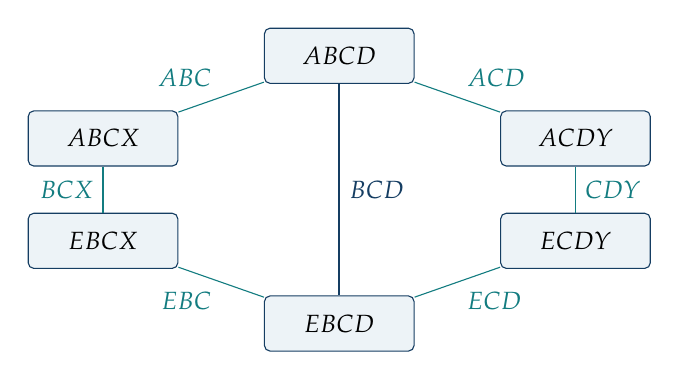
\begin{tikzpicture}[every node/.style={font=\small},
  cell/.style={draw=inkblue,rounded corners=2pt,fill=lightblue,minimum width=19mm,minimum height=7mm}]
\node[cell] (a) at (0,0) {$ABCD$};
\node[cell] (b) at (0,-3.4) {$EBCD$};
\node[cell] (x) at (-3,-1.05) {$ABCX$};
\node[cell] (z) at (-3,-2.35) {$EBCX$};
\node[cell] (y) at (3,-1.05) {$ACDY$};
\node[cell] (w) at (3,-2.35) {$ECDY$};
\draw[inkblue,thick] (a)--node[right]{$BCD$}(b);
\draw[teal] (a)--node[above left]{$ABC$}(x);
\draw[teal] (x)--node[left]{$BCX$}(z);
\draw[teal] (z)--node[below left]{$EBC$}(b);
\draw[teal] (a)--node[above right]{$ACD$}(y);
\draw[teal] (y)--node[right]{$CDY$}(w);
\draw[teal] (w)--node[below right]{$ECD$}(b);
\end{tikzpicture}
\caption{The original dual graph of the sharp ball. Each labelled edge is
an internal paired triangle. The only internal primal edges are $BC$ and
$CD$, both of degree four. The central upward move enables two downward
moves, whose union consumes every original tetrahedron.}
\label{fig:gadget}
\end{figure}

\begin{proposition}[Sharpness at one upward move]\label{prop:sharp}
The ball \eqref{eq:gadget} has no initial downward move. It admits a descent
using one upward and two downward moves, but every descent using at most
one upward move consumes all six original tetrahedra. Thus the value
$3U+3=6$ cannot be reduced to five at $U=1$ in the stated move model.
\end{proposition}
\begin{proof}
The only internal edges are $BC$ and $CD$, each with four incident
tetrahedra. Therefore no downward move is initially legal. An upward move
through $BCD$ replaces the central two tetrahedra by
$AEBC,AECD,AEDB$. The edge $BC$ now supports a downward move using
$AEBC,ABCX,EBCX$, producing $AEBX,AECX$. The edge $CD$ supports the second
downward move using $AECD,ACDY,ECDY$, producing $AECY,AEDY$. Five tetrahedra
remain. The two downward moves commute in this displayed construction.

For the lower bound, a first descent with at most one upward move must have
the pattern up/down/down. The upward move creates one new internal edge.
If the first downward move deletes that edge, it undoes the upward move
and returns to a triangulation with no downward move. Otherwise it deletes
$BC$ or $CD$. To reduce that edge's degree from four to three, the upward
move must have used it in its central triangle. Its ensuing downward move
consumes exactly one of the three new tetrahedra and produces two tetrahedra
containing the newly created edge. That new edge's degree therefore changes
from three to four and it cannot be deleted by the second downward move.
The second move must delete the other of $BC,CD$.

An untouched original tetrahedron incident to an edge prevents that edge
from disappearing. Hence deleting both edges forces consumption of the
union of their original stars, which is precisely all six tetrahedra.
\end{proof}

The accompanying independent Regina inventory examines every first upward
move: seven candidates, fifteen up/down prefixes, and four successful
up/down/down traces. Their first faces are $BCD$ (two orders), $BCX$, and
$CDY$; all have footprint six. The initial and final isomorphism signatures
are respectively \code{gbbjrcadfaa} and \code{fbbfiaev}. These finite records
check the construction and the proof's edge inventory; they are not used to
infer an asymptotic statement from a few examples. The article claims sharpness
at $U=1$, not asymptotic optimality of the coefficient three for all $U$.

\section{A category boundary: strict simplicial moves}

The hypotheses about generalized triangulations cannot be omitted. Let $S$
be the boundary of an octahedron and form its simplicial suspension with
vertices $x,y$. This triangulates a $3$-sphere. For each base triangle $abc$,
the tetrahedra $xabc,yabc$ admit a strict simplicial $2$--$3$ move because
the proposed edge $xy$ is initially absent.

Choose two opposite base triangles. Their two move supports are disjoint,
and both moves are initially legal. Performing either creates the edge
$xy$, so the other is then forbidden by the strict simplicial nonexistence
condition for the new simplex. Disjoint consumed tetrahedra therefore do
not imply commutation in that category. Reversing the first move gives a
backward-persistence failure caused by deletion of a global obstruction,
without consumption of any tetrahedron used by the newly enabled move.

The repository's generalized model allows distinct edges with the same
global endpoints and has no such absent-simplex condition. Extending the
theorem to a different move model requires recording its additional
dependencies and reproving the locality bound.

\section{Complete fixed-parameter simplification}\label{sec:complexity}

\subsection{Constructively enumerating connected regions}

For completeness, we give the combinatorial ingredients of the incoming
region bound explicitly. This separates the new localization theorem from
the search machinery on which its stronger algorithmic consequence rests.

\begin{lemma}[Connected-region count]\label{lem:regions}
In a graph with $t$ vertices and maximum degree four, the number of connected
$i$-vertex sets is at most $t16^{i-1}$ for $i\ge1$. All connected sets of
size at most $R$ can be enumerated without repetition using polynomial work
per generated set.
\end{lemma}
\begin{proof}
Choose the least vertex as root and a deterministic spanning tree of each
connected set. A depth-first traversal of the tree has $2(i-1)$ edge steps.
Record the root and, at each step, one of at most four local neighbour ports.
The walk reconstructs its visited vertex set, so this is an injective
encoding among the deterministic choices. There are at most
$t4^{2(i-1)}$ such encodings.

To enumerate sets, define the parent of a non-singleton connected set $A$
by deleting its largest non-root vertex whose deletion leaves a connected
set. A spanning tree has a leaf other than the root, so at least one deletion
exists. Iterating the parent reaches the singleton root. From each current
set, consider its at most $4|A|$ frontier neighbours and accept an extension
exactly when its canonical parent is the current set. This visits each set
once. Testing all candidate deletions and their connectivity uses only
polynomial work in $|A|$. An explicit stack gives the implementation without
recursion-depth dependence on the ambient number of vertices.
\end{proof}

The geometric factor $t$ chooses the location of the region. It is not
raised to a power proportional to $U$. This is the step that direct
enumeration of all $R$-subsets would lose.

\subsection{An elementary independent FPT bound}

Before using commutation compression, localization alone already implies
fixed-parameter tractability. In a region containing $i$ original cells,
at most $i+U$ eligible cells are live at any time. A legal eligible event
is specified by a local face or edge of such a cell; there are at most
$10(i+U)$ choices before eliminating repetitions and illegal configurations.
Every first-descent witness has at most $2U+1$ events. Thus direct local
branching, followed over every connected region of size at most $3U+3$,
gives
\begin{equation}\label{eq:elementary-fpt}
 2^{O(U\log(U+2))}\poly(t+B).
\end{equation}
This proof supplies a separate, weaker FPT guarantee that does not require
the constant-alphabet trace theorem. The sharper result below removes the
extra $\log U$ in the exponent.

\subsection{Constant-alphabet encoding of commuting traces}

Assign each eligible incarnation a commitment from
\begin{equation}\label{eq:alphabet}
 \mathcal A=\{\mathrm{idle}\}\ \cup\
 \{\mathrm{down\ at\ edge}\ e:0\le e<6\}\ \cup\
 \{\mathrm{up\ at\ face}\ f:0\le f<4\}.
\end{equation}
An event is ready if all its participants choose their local port for that
event. Two different ready events cannot share an incarnation: a local face
determines its unique paired-face event, and a local edge determines its
unique full edge-star event. Ready events therefore commute by
\cref{lem:forward}.

Fix a deterministic scheduler. If an event is ready, execute the first ready
event; otherwise assign the next unassigned eligible incarnation one of its
eleven symbols. Surviving cells retain their commitments; born cells are
unassigned. Protected original cells are permanently idle.

\begin{lemma}[Commitment encoding]\label{lem:encoding}
For a supplied region with $i$ original cells, every finite trace using
$u$ upward and $d$ downward events has an encoding of length
$i+3u+2d$ over \eqref{eq:alphabet}, up to interchanges of independent events.
Consequently the number of commuting classes with $u\le U$ and
$d\le u+1$ is at most
\begin{equation}\label{eq:descent-count}
 11^{i+5U+2}.
\end{equation}
The generic bounded-region family, without the latter loss restriction,
has at most $11^{3i+5U}$ classes.
\end{lemma}
\begin{proof}
For a target trace, give each incarnation the port of the event that
eventually consumes it, and give every target survivor the symbol idle.
Follow these choices when the deterministic scheduler asks for them.

If an event is ready, consider the first remaining target event touching
one of its source incarnations. All earlier events leave those sources
intact. Its commitment identifies exactly that ready event, so the first
touch must be the ready event itself. All preceding target events have
disjoint consumed supports; the persistence and relative-boundary lemmas
move the ready event to the front. Iterating realizes the target trace
up to commuting independent events. Assigning the recorded symbols cannot
stop before the next target event is ready, and target survivors are idle.

The freely assigned incarnations comprise the $i$ eligible originals and
the $3u+2d$ born cells. Each receives one symbol. Record assignments in the
order requested by the deterministic scheduler. Padding by idle symbols
to a common maximum length preserves an injective encoding of trace
classes: decoding a word determines one execution. Substituting
$d\le u+1$ yields \eqref{eq:descent-count}. In a general region-supported
trace, protected originals survive, so $d\le i+u$, giving the final bound.
\end{proof}

The counting decoder in this lemma is allowed to pass an earlier descent
introduced by reordering. It need not follow the implementation's early-stop
policy. The target trace's event counts and total encoding length are what
establish the injection. Confusing these two roles would unnecessarily weaken
or invalidate the counting argument.

The practical search uses sleep sets instead of literal assignments. It
explores enabled events in deterministic order and remembers an earlier
sibling event across a later branch only while its consumed incarnation
set is disjoint from each intervening event. Once a source incarnation is
destroyed it never reappears. This nonresurrection, local event uniqueness,
and persistence imply that at most one representative of a commuting class
is visited. Conversely, the first representative of each class in the fixed
search order cannot be blocked: a blocking event could be commuted left to
obtain an earlier representative. This is the exact finite sleep-set argument
specialized to these geometric events, as implemented in the incoming engine
\cite{incoming-trace}.

\begin{theorem}[Complete bounded-upward descent]\label{thm:fpt}
For a valid generalized source $T$ of size $t\ge1$, an optional integral
marking of input bit bound $B$, and $U\ge0$, question \eqref{eq:decision}
is decidable in
\begin{equation}\label{eq:fpt}
 t\,2^{O(U)}\poly(t+U+B)=2^{O(U)}\poly(t+B)
\end{equation}
bit operations. A positive answer supplies a geometrically replayable
first-descent trace. No spatial-coverage hypothesis is required.
\end{theorem}
\begin{proof}
Set $R=\min(t,3U+3)$. Enumerate all connected original regions of size at
most $R$ and search their bounded-upward traces with the endpoint predicate
$|T'|<t$. A positive test returns immediately. If no positive is found,
every permitted family is exhausted. The localization theorem proves that
this decides \eqref{eq:decision} completely.

Every visited prefix before success has $d\le u$, and the first successful
one has $d=u+1$. Combining \cref{lem:regions,lem:encoding}, a sufficient
counting factor, including the source endpoint, is
\begin{equation}\label{eq:explicit-count}
 1+t\sum_{i=1}^{R}16^{i-1}11^{i+5U+2}.
\end{equation}
Since $R\le3U+3$, this is $t2^{O(U)}$ times a fixed constant. In particular,
the largest commitment exponent is $8U+5$, improving the $14U+9$ obtained
by substituting $R$ into the generic region bound. The bit analysis below
supplies polynomial work per visited encoding or representative. It includes
the endpoint count test. This proves \eqref{eq:fpt}.
\end{proof}

\begin{corollary}[Small-budget regimes]\label{cor:qp}
Bounded-upward descent is polynomial-time when $U=O(\log(t+2))$, and takes
$t^{O(\log(t+2))}\poly(B)$ time when $U=O(\log^2(t+2))$.
\end{corollary}
\begin{proof}
Substitute the budget into \eqref{eq:fpt}. Polynomial factors in $U$ are
absorbed by the indicated bounds. The bit bound $B$ remains polynomially
charged.
\end{proof}

The constants in \eqref{eq:explicit-count} are intentionally conservative.
It is an asymptotic guarantee, not a prediction that large $U$ is practical.
For $U=0$, the problem is simply the existence of a legal initial downward
move, since any descending trace has a first downward move. Directly checking
edge stars solves that special case without a general region enumeration.

\subsection{Binary arithmetic and certificate size}

\begin{lemma}[Upward moves control marking growth]\label{lem:bits}
Let $D_0$ be the maximum absolute source edge value. After a trace with $u$
upward events, all signed edge values have magnitude at most $2^uD_0$.
Normalized height rows and local coherent normal coordinates have bit
length at most $B+u+O(1)$.
\end{lemma}
\begin{proof}
A downward move removes one edge and creates no new edge; all surviving
edge values remain unchanged. The new diagonal of an upward move joins
the two formal apices $a,b$. Through any belt vertex $v$, its value is
$(h_b-h_v)+(h_v-h_a)$, a sum of two old signed edge values. Its magnitude
is at most twice the previous maximum, and all other edge values persist.
Induct on $u$. A normalized row entry is an edge difference from its first
corner. A local normal coordinate is a gap between ordered corner heights,
bounded by their span, which is itself an edge difference.
\end{proof}

There are $O(t+U)$ local edge and face occurrences at every visited state.
Global manifold validation, grouping edge stars, comparing local patterns,
and copying a full triangulation therefore cost polynomial time in
$t+U+B$. The code currently rebuilds global geometry where needed; it makes
no constant-time local-update claim. Stable incarnation names are exact
interned DAG expressions, not cryptographic identity assumptions.

A first-descent proof with complete intermediate snapshots has bit length
\begin{equation}\label{eq:certificate-size}
 O\bigl((U+1)(t+U)(B+U+\log(t+U+1))\bigr).
\end{equation}
It contains at most $2U+1$ moves, each with at most $t+U$ rows, plus the
final coordinate data. Independent replay is polynomial in this size.
Exhaustive failure is an algorithmic conclusion about a bounded family;
the implementation does not claim a comparably short negative certificate.

\subsection{Repeated bounded simplification}

\begin{definition}
A triangulation is $U$-irreducible for this move model if it admits no
strict descent using at most $U$ total upward moves.
\end{definition}

\begin{corollary}[Complete bounded preprocessing]\label{cor:preprocess}
Repeatedly applying complete bounded-$U$ descent and adopting each verified
positive result terminates at a $U$-irreducible triangulation in
$2^{O(U)}\poly(t+B)$ bit time. Its concatenated positive proof uses at most
$tU$ upward events and $t(2U+1)$ events in total.
\end{corollary}
\begin{proof}
Each successful restart reduces the tetrahedron count by at least one,
so there are fewer than $t$ successful restarts. Each local transient state
has at most $t+U$ tetrahedra. Across all successful traces, \cref{lem:bits}
increases the marking bit bound by at most $tU+O(1)$. Summing the polynomial
overheads in \cref{thm:fpt} gives the stated bound. The final complete
negative bounded search is precisely the definition of $U$-irreducibility.
\end{proof}

An arbitrary choice of successful one-unit descents is not guaranteed to
preserve a prescribed total upward budget for a later $k$-unit objective.
The next section treats that joint-budget problem separately.

\section{Several units of descent and color coding}\label{sec:multiunit}

The connected witness theorem answers one-unit descent. Requiring a decrease
by at least $k$ tetrahedra may require several independent regions. Their
locations need not be enumerated with a $t^k$ factor: their total original
footprint remains bounded, which permits standard deterministic color coding.
This section gives a further algorithmic theorem. The delivered code includes
the exact packing primitive for a supplied coloring and finite audits; it does
not implement the full deterministic perfect-hash-family construction.

\begin{theorem}[Multiunit localization]\label{thm:k-local}
Suppose a trace with at most $U$ upward events reduces $T$ by at least
$k\ge1$ tetrahedra. Then there is such a trace with $u\le U$, $d=u+k$,
length $2u+k$, and at most $k$ birth components. Each component has positive
loss and connected actual original footprint. Their disjoint union has size
at most $3U+3k$.
\end{theorem}
\begin{proof}
Choose a shortest trace meeting the threshold. It first reaches loss $k$
at its final event, so $d=u+k$. If a component had nonpositive loss, deleting
it using \cref{thm:projection} would preserve loss at least $k$ and shorten
the trace. All component losses $\ell_j$ are therefore positive integers,
with $\sum_j\ell_j=k$, so the number $c$ of components is at most $k$.
Their footprints are disjoint and connected by \cref{lem:connected}. Summing
\cref{lem:incidence} yields
\[
 |F|\le u+2d+c=3u+2k+c\le3U+3k.
\]
\end{proof}

\begin{lemma}[Composing disjoint original footprints]\label{lem:compose}
Let $\sigma_1,\ldots,\sigma_s$ be legal traces from the same marked source
whose actual original footprints are pairwise disjoint. They can be replayed
in any order, transporting the exterior attachments at each step. The
combined upward cost and tetrahedron loss are the sums of the individual
costs and losses.
\end{lemma}
\begin{proof}
Give births in different traces disjoint names. Every incarnation consumed
by one trace is either one of its original footprint cells or a birth
descended from those cells. Distinct traces therefore have disjoint consumed
incarnation sets after transport. At the common source their first events
are simultaneously legal and commute. Inductively construct the grid of
interleavings: at every square, \cref{lem:forward} transports the next event
of either trace across the next event of the other, retaining the same
relative-boundary attachments. This proves that both complete orders are
legal. Apply the two-trace argument repeatedly. Marking agreement follows
from the same local transport lemma, and the count assertions follow by
adding event counts.
\end{proof}

This lemma does not require an actual footprint to be a ball or an induced
subcomplex with embedded closure. Individual formal replacements, with their
boundary ports, are the units of the proof. It also does not claim that
arbitrary traces with overlapping original footprints compose.

\subsection{Enumerating candidate items}

Set $p=\min(t,3U+3k)$. Over every connected original cover of size at most
$p$, enumerate the full bounded-upward region family and retain every
positive-loss endpoint. Each item $j$ records
\[
 (A_j,a_j,b_j,\sigma_j),
\]
Here $A_j$ is its \emph{actual} consumed original footprint, $a_j\le U$
is its upward cost, and $\sigma_j$ is a replayable source-bound trace.
The positive profit is capped: $b_j=\min(k,\loss(\sigma_j))$. The total item
count and generation cost are bounded by
\begin{equation}\label{eq:items}
 M\le t\,2^{O(p+U)}\poly(t+U+B).
\end{equation}
This is the generic connected-region commitment bound. A particular actual
footprint can appear under several covers; retaining duplicate items does
not affect the upper bound or correctness.

The item generator must continue through intermediate descents. Calling a
first-descent routine and collecting only its first answer would not enumerate
the needed component alternatives. Birth-connectedness need not be tested
for every retained item: extra legal items remain sound, while every component
of the minimum witness in \cref{thm:k-local} is necessarily represented.

\subsection{Colorful packing with original witnesses}

A family $\mathcal H$ of functions $[t]\to[p]$ is $p$-perfect if every subset
of at most $p$ source indices is mapped injectively by at least one member.
The standard deterministic construction of Naor, Schulman, and Srinivasan
has size $e^p p^{O(\log p)}\log(t+2)$ and total construction time bounded by
$2^{O(p)}\poly(t)$ \cite{nss}. We need this total-time statement; we do not
assume a constant-delay hash enumerator. Color coding itself is classical
\cite{color-coding}; an explicit modern treatment of the stronger delay
requirements is available in \cite{gutin-color}.

For a fixed coloring $h\in\mathcal H$, discard an item if $h$ is not
injective on $A_j$. Otherwise store its nonempty color mask
$C_j=h(A_j)\subseteq[p]$. Use the following ordinary $0/1$ dynamic program:
\begin{align*}
 D_0(\varnothing,0)&=0,\qquad D_0(S,a)=-\infty\text{ otherwise},\\
 D_j(S,a)&\gets D_{j-1}(S,a),\\
 D_j(S\cup C_j,a+a_j)&\gets
 \max\{D_j(S\cup C_j,a+a_j),\min(k,D_{j-1}(S,a)+b_j)\}
\end{align*}
for every finite state with $S\cap C_j=\varnothing$ and $a+a_j\le U$.
The state value is the best capped total loss from the first $j$ items,
using exactly mask $S$ and upward cost $a$. Take/skip predecessor data
retains actual item identities for reconstruction; a linear combination of
traces is never treated as a geometric witness.

The number of states is $2^p(U+1)$, and a direct item scan costs
$O(M2^p(U+1))$. Positive items have nonempty footprints, so the empty-mask
degeneracy does not arise. Mask disjointness implies actual source-cell
disjointness, even though distinct source cells may share colors. By
\cref{lem:compose}, a successful collection is geometrically replayable and
has total upward cost at most $U$ and loss at least $k$.

\begin{theorem}[Fixed-parameter multiunit descent]\label{thm:k-fpt}
For generalized formal-bipyramid moves, existence of a trace with at most
$U$ total upward moves reducing a valid $t$-tetrahedron source by at least
$k$ tetrahedra is decidable deterministically in
\begin{equation}\label{eq:k-fpt}
 2^{O(U+k)}\poly(t+B)
\end{equation}
bit time. A positive result admits a source-bound geometric trace certificate.
\end{theorem}
\begin{proof}
Trivial impossible thresholds, including $k\ge t$ for a nonempty connected
source, may be answered directly. In the remaining cases construct the
items above and run the packing dynamic program for every coloring in
$\mathcal H$. Soundness follows from \cref{lem:compose}.

For completeness, take the minimum-length witness of \cref{thm:k-local}.
Its component footprints are individually connected, pairwise disjoint,
and their union has at most $p$ vertices. Each component trace occurs among
the items. Some $h\in\mathcal H$ colors the entire union injectively, so
these items have pairwise disjoint color masks. Their upward costs sum to
at most $U$ and their profits sum to $k$; the dynamic program finds a
successful collection. Enumerating every coloring therefore decides the
question completely.

Multiply \eqref{eq:items}, the $2^p(U+1)$ dynamic-program factor, and the
$2^{O(p)}\log(t+2)$ hash-family factor. Since $p\le3(U+k)$, the result is
\eqref{eq:k-fpt}, with polynomial source and replay costs included.
\end{proof}

The weaker direct alternative is to enumerate covers with up to $k$
components, which gives $t^k2^{O(U+k)}\poly(t+U+B)$. The color-coding
argument removes the $t^k$ factor. This is a consequence of the new bounded
total footprint and independent replay, composed with an established
derandomization theorem. It is not a claim that color coding is new.

With $U+k=O(\log t)$ the decision problem is polynomial; with
$U+k=O(\log^2 t)$ it is quasi-polynomial. The supplied-coloring prototype
tests the witness-preserving packing step, while \cref{thm:k-fpt} relies
on the cited complete perfect-family construction for deterministic
exhaustion over all possible locations.

\section{One exact search over overlapping covers}\label{sec:implementation}

The localization theorem makes the old spatial search complete for descent,
but independent restarts still repeat substantial work. A source with many
small overlapping covers can revisit the same marked trace prefix once for
each cover containing its footprint. The new implementation represents the
union of those finite search languages directly.

\subsection{The cover intersection invariant}

Let $\mathcal R$ be the complete family of permitted original regions,
including the empty region. For each original tetrahedron $v$, build the
inverted incidence list
\[
 I(v)=\{R\in\mathcal R:v\in R\}.
\]
A search frame with actual footprint $F$ retains precisely
\begin{equation}\label{eq:cover-intersection}
 C(F)=\{R\in\mathcal R:F\subseteq R\}
     =\bigcap_{v\in F} I(v).
\end{equation}
The empty intersection means all covers. The implementation represents that
root case by a sentinel instead of copying the complete index. If an event
first consumes the original cells in $S$, its compatible covers become
\[
 C(F\cup S)=C(F)\cap\bigcap_{v\in S}I(v).
\]
An empty result rejects that branch. Consuming a born cell adds no new
original identity: its ancestors already entered the footprint at their
own first consumption. Intersections begin with the smallest available
incidence set, reducing intermediate allocations without changing the set.

\begin{proposition}[Exact union language]\label{prop:union}
The indexed cover search permits exactly the traces admitted by at least
one independently restarted search over $\mathcal R$. It preserves the
relative commutation equivalence used by the sleep-set search.
\end{proposition}
\begin{proof}
Induction on the trace length proves \eqref{eq:cover-intersection}. A trace
is admitted exactly when some region contains every consumed original cell,
which is the definition of membership in the union of the restarted
languages. Every prefix consumes a subset of that final footprint, so it
is admitted under the same covering region.

For two adjacent independent events in an admitted trace, either order has
the same final footprint, while the two intermediate footprints are subsets
of it. The same cover therefore admits both orders. Their geometry and
markings agree by \cref{lem:forward}. Thus all swaps required by the
sleep-set argument remain within the union language.
\end{proof}

Two events may be individually allowed at a prefix although their combined
footprint fits no cover. The proposition does not assert that every such
pair can be combined. It asserts commutation when the whole two-event trace
is admitted, which is exactly the property the reduction needs.

An explicit index has at most $\sum_{R\in\mathcal R}|R|$ incidences. For
connected radius $R_0=O(U)$ this is $t2^{O(U)}$ times a polynomial parameter
factor. Intersecting finite sets and copying compatible-cover states keeps
the same fixed-parameter time form, although it can consume more memory
than streaming one region at a time. The theorem does not promise that a
fully materialized index is the best implementation for every input.

There is also a sharper accounting for cover intersections. Let $C_f$ be
the compatible-cover set at visited frame $f$, and let $K_R$ bound the
commuting trace classes admitted by a fixed cover $R$. Then
\[
 \sum_f |C_f|
 =\sum_{R\in\mathcal R}\#\{f:R\in C_f\}
 \le\sum_{R\in\mathcal R}K_R.
\]
For a fixed cover, the global sleep search still visits at most one
representative of each admitted class. An intersection can scan the smaller
set; ordered incidence tables with binary search give a deterministic
logarithmic overhead per tested membership. Thus incidence work can be
charged to compatible cover/frame pairs instead of multiplying every
frame by the size of the entire region family. The prototype uses exact
Python sets, with equality resolving hash collisions.

\subsection{Lazy transitions and endpoint observations}

Each queued branch stores its parent state and the proposed geometric event.
The native replacement and integral cochain transport are performed only
when that branch is visited. A positive early answer can therefore avoid
constructing all unused siblings. The node limit is checked before producing
the next unvisited child. This matters on the upward-required fixtures:
the source has many upward choices, while a successful trace uses only
three events.

Exact marked endpoint keys suppress repeated endpoint queries. They retain
the source incarnation identities and transported cochain, using exact
interned structures rather than probabilistic hash equality. The search
does \emph{not} delete continuation frames merely because an endpoint query
was already made. Remaining upward budget, sleep obligations, and compatible
covers can differ between histories reaching similar geometry. Proving a
safe stronger quotient is a separate problem.

A complete conclusion for a caller's predicate requires that predicate to
be invariant under the represented marked endpoint and commuting trace
equivalence. A callback that inspects the particular certificate history
or arbitrarily selected witness cover is outside that guarantee. Strict
tetrahedron descent and the supplied-vector disc predicate have the required
invariance.

The finite-family cost separates three tasks: construction of the complete
cover index, exploration of geometric traces, and evaluation of endpoints.
The descent endpoint test is just a tetrahedron count. A normal-disc query
is optional and has its own potentially substantial cost. Performance
claims for the descent test therefore do not automatically transfer to an
arbitrary disc-search callback.

\subsection{Public interfaces and exact meanings of results}

The generic entry point is \code{search_pachner_cover} in
\code{fastunknot/pachner_cover_search.py}. It accepts a source triangulation
and height rows, a maximum region size, maximum number of components,
total upward budget, and explicit resource limits. The methods are the
maintained sleep-set route and a small-instance naive reference route.
The older restarted and commitment implementations remain available.

The convenience entry point \code{find_pachner_descent} supplies the
radius $\min(t,3U+3)$ unless the caller explicitly requests another radius.
It queries strict tetrahedron loss and independently verifies a positive
answer. A smaller requested radius is a legitimate local search, but its
failure has a deliberately narrower status.

\begin{table}[ht]
\centering\small
\begin{tabularx}{\textwidth}{@{}p{0.39\textwidth}X@{}}
\toprule
Status & Meaning \\
\midrule
\code{DESCENT_FOUND} & Source replay verifies strict descent and the declared
total upward bound. \\
\code{COMPLETE_BOUNDED_DESCENT} & No descent exists within that upward budget,
using the sufficient localization radius and complete search. \\
\code{COMPLETE_BOUNDED_LOCAL_DESCENT} & Only the explicitly smaller covered
family is exhausted. \\
\code{COMPLETE_BOUNDED_COVER_FAMILY} & The complete declared generic cover
family is exhausted. \\
\code{INCONCLUSIVE} & A required index, traversal, replay, or endpoint-query
operation reached its limit. \\
\bottomrule
\end{tabularx}
\caption{The principal search outcomes. Exhaustion is a bounded geometric
conclusion and is not a nontrivial-knot certificate.}
\label{tab:statuses}
\end{table}

The generic interface also distinguishes an independently verified normal-disc
answer, \code{DISC_FOUND}, from a caller-selected endpoint,
\code{ENDPOINT_SELECTED}. A certificate on an abstract manifold still needs
the maintained diagram-to-exterior binding before it can certify a statement
about a supplied knot diagram.

\begin{lstlisting}[language=Python,float=htbp,caption={Complete bounded descent with an independently checked positive witness.}]
from fastunknot.pachner_cover_search import find_pachner_descent
from fastunknot.pachner_cover_verify import verify_pachner_descent

answer = find_pachner_descent(
    triangulation, heights, max_upward=1,
    max_nodes=10000, max_regions=100000, max_work=2000000,
)
if answer["status"] == "DESCENT_FOUND":
    assert verify_pachner_descent(
        triangulation, heights, answer["certificate"],
        max_upward=1,
    )
\end{lstlisting}

\subsection{Independent certificate checking}

The producer emits the existing
\code{pachner-cochain-endpoint-v1} schema. Its declared active original
region is one concrete member of the compatible-cover set; it need not
equal the actual consumed footprint. The new verifier independently checks
that this cover has the stated size and number of induced dual components,
then invokes the maintained source-bound geometric and cochain replay.
It imports no region enumerator, search engine, native move producer, or
cochain-transport producer.

For descent, it also recomputes upward and downward counts, checks the
actual final tetrahedron count, and verifies
$t_{\rm final}=t_{\rm initial}+u-d<t_{\rm initial}$. This prevents the
search's status string or claimed counters from substituting for a proof.
The verification tests disable the corresponding producer functions and
still accept genuine retained certificates.

Resource caps are part of the observable contract. \code{max_regions}
limits construction of the \emph{complete} index, including the empty
region. Partial construction cannot establish complete exhaustion.
\code{max_nodes} counts visited search frames; \code{max_work} counts
cooperative checkpoints across preparation, indexing, search, and positive
replay. These checkpoints are operational accounting units, not bit
operations. Optional disc-query caps also prevent a complete disc-negative
claim when a required query was unfinished. User callback exceptions
propagate unchanged, including exceptions whose class happens to match an
internal budget exception. Callback inputs are isolated from mutable search
state.

\section{Certificate projection, composition, and packing}\label{sec:certificate-tools}

\subsection{Extracting a connected first descent}

The new \code{pachner_causality.py} reads a supplied endpoint proof only
after independent source replay accepts it. Each live tetrahedron receives
either a source identity or a pair consisting of its birth event and output
slot. Reading the consumed regions recovers every birth arc and the actual
source footprint. The analyzer reports the components, their losses, and
the incidence census.

For a descending certificate, \code{extract_local_descent} chooses a
positive-loss component, projects its events, and truncates at first
descent. These operations repeat until the retained trace is connected
and first-descending. One projection followed by one truncation is
insufficient: deleting a late event that joined earlier components can
disconnect the prefix again. Every necessary repetition strictly shortens
the trace, giving termination. The final witness satisfies the localization
bound and is independently replayed before return.

The consumer must respect every local frame accepted by the public verifier.
A valid downward certificate can use either order for two belt vertices in
the seed tetrahedron. A native producer may choose just one order. Replaying
with that producer's frame and then treating its born tetrahedra as if they
used the declared frame corrupts later dependent events, even though the
first replacement has the right unmarked geometry. The extractor therefore
retains the declared formal region and, where necessary, relabels the two
born tetrahedra and all incident permutations before carrying the cochain.
This fix is exercised by a retained noncanonical-frame counterexample and
an exhaustive finite frame audit described in \cref{sec:experiments}.

\subsection{Composing independently supplied traces}

The companion \code{compose_disjoint_traces} authenticates every input
endpoint against the same original source. It computes \emph{actual}
consumed footprints and rejects intersecting ones, even if their advertised
cover regions happen to differ. Birth names are namespaced by input trace,
so equal event numbers from different certificates cannot collide. The
replay transports source and birth identities, preserving declared formal
frames, and returns one ordinary source-bound endpoint certificate together
with the additive count census. This is an executable positive-witness
counterpart of \cref{lem:compose}. Overlapping supplied covers are harmless
when the actual footprints are disjoint.

The function does not assume that input traces are descending. The geometric
composition lemma applies to arbitrary legal traces with disjoint actual
footprints; a caller may separately inspect their losses. Empty traces are
allowed and contribute zero. Invalid proofs, overlap, or exhausted work
do not produce a partial successful composition.

\subsection{The supplied-coloring dynamic program}

The prototype \code{causal_research/colorful_packing.py} implements the
exact $0/1$ packing step of \cref{sec:multiunit} for a supplied coloring.
It validates nonempty distinct-source footprints, nonnegative upward costs,
and positive losses. It discards noncolorful items, compacts unused numeric
color labels, and preserves original candidate indices in immutable witness
tuples. A separate previous-item table prevents accidental reuse of an item.

Its objective is maximum capped loss, followed by minimum upward cost.
It does not claim globally minimum witness cardinality or lexicographically
first item indices: retaining only one best capped profit per mask and
cost does not justify those extra objectives. The result exposes actual
loss as well as capped loss, upward cost, union footprint, and color mask.
The candidate dictionaries can retain authenticated certificates, but the
combinatorial routine itself does not authenticate their geometry.

The delivered prototype does not generate the complete deterministic
perfect-hash family. Consequently a negative result from one coloring
is only a negative result for that colorful item instance. The mathematical
algorithm in \cref{thm:k-fpt}, the implemented packing primitive, and the
independent positive composition utility are separate, explicit deliverables.

\section{Experimental evidence and its limits}\label{sec:experiments}

The experiments test equivalence of bounded searches, independent replay,
the default localization radius, and the cost of repeated overlap. They
do not measure a complete knot-recognition pipeline. All raw data, source
digests, generated fixtures, and replay commands are retained.

\subsection{Genuine upward-required solid-torus fixtures}

Start with a one-tetrahedron layered solid torus and attach a chain of $g$
copies of the six-tetrahedron ball along boundary triangles. Attaching a
ball along a boundary disc preserves the solid torus. The resulting source
has $t=6g+1$ tetrahedra. Its cocycle is computed and validated using the
maintained exact native routines. Independent Regina checks confirm validity,
orientability, and the solid-torus type for the controlled small instances
\cite{regina}.

These sources have no initial downward move; the native move inventory has
$8g$ upward choices. A local first descent requires one upward and two
downward moves and consumes six original gadget cells. For the one-gadget
source the complete $U=0$ test fails to descend, and the complete
$U=1,r=5$ covered search also fails. With $U=1,r=6$, the native search
returns an independently accepted descent. This distinguishes a genuinely
upward-required test from an example solved by an initial greedy collapse.
The separate ball proof and Regina inventory establish the sharper
radius statement of \cref{prop:sharp}.

\subsection{Matched timing protocol}

The retained measurements use Python 3.12.14 on
\code{Linux-6.18.44-x86_64-with-glibc2.39}. Every source is constructed once.
The independent controls use Regina engine 7.4 (Python package 7.4.1).
Both routes use the same $U=1,r=6$, cochain, native move and transport
routines, and relevant resource limits. Disc queries are disabled.
Each reported time is the median of three retained samples; the run order
alternates between restarted and shared search. The speed ratio is the
ratio of those two medians, not the median of per-pair ratios.

For complete-family timings, endpoint collection is disabled in both
routes. Endpoint equality is checked separately. For first-descent timings,
both routes include the same independent positive verifier. Source fixture
construction is outside the timed calls, while region enumeration and
index construction are inside. Timing uses a shared execution environment,
without dedicated CPU isolation. Three samples document a reproducible
finite comparison but do not support a population confidence interval or
an extrapolated running-time law.

\begin{table}[ht]
\centering\small
\begin{tabular}{@{}rrrrrrrr@{}}
\toprule
$t$ & Covers & \multicolumn{2}{c}{Visited frames} &
\multicolumn{2}{c}{Median seconds} & Ratio & Endpoints\\
\cmidrule(lr){3-4}\cmidrule(lr){5-6}
& & Restart & Shared & Restart & Shared & & \\
\midrule
7  & 66  & 495  & 28 & 1.15956  & 0.09137 & $12.69\times$ & 14\\
13 & 334 & 3152 & 55 & 13.39354 & 0.22377 & $59.85\times$ & 27\\
\bottomrule
\end{tabular}
\caption{Complete covered-family exhaustion. ``Endpoints'' counts exact
signed-cochain geometric isomorphism classes, checked outside the timed
runs. The shared search retains more marked representatives.}
\label{tab:exhaustion}
\end{table}

\begin{table}[ht]
\centering\small
\begin{tabular}{@{}rrrrrrr@{}}
\toprule
$t$ & Covers & \multicolumn{2}{c}{Visited frames} &
\multicolumn{2}{c}{Median seconds} & Ratio\\
\cmidrule(lr){3-4}\cmidrule(lr){5-6}
& & Restart & Shared & Restart & Shared & \\
\midrule
7  & 66   & 273 & 6 & 0.71148  & 0.01801 & $39.50\times$\\
13 & 334  & 630 & 6 & 2.75100  & 0.03303 & $83.29\times$\\
25 & 934  & 641 & 6 & 6.03841  & 0.10123 & $59.65\times$\\
49 & 2134 & 641 & 6 & 10.68172 & 0.14371 & $74.33\times$\\
\bottomrule
\end{tabular}
\caption{First independently verified strict descent on the controlled
solid-torus family. Every selected witness uses one upward and two downward
moves. These are simplifier measurements, not end-to-end unknot timings.}
\label{tab:descent}
\end{table}

\begin{figure}[ht]
\centering
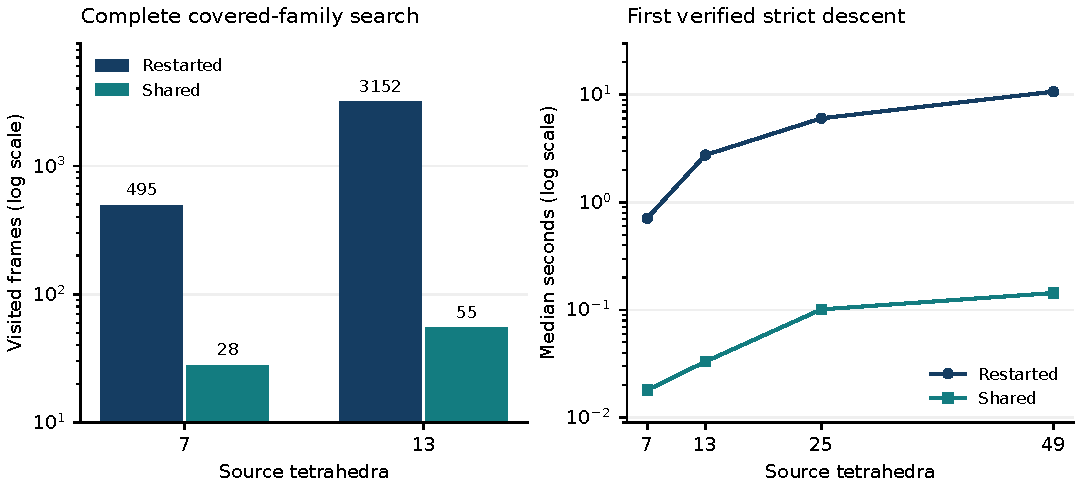
\includegraphics[width=\textwidth]{figures/benchmarks.pdf}
\caption{Two views of the same retained data. Logarithmic vertical axes
make the smaller shared-search counts and times legible. Lines connect
the four measured first-descent cases and do not represent a fitted
asymptotic model.}
\label{fig:benchmark}
\end{figure}

In the complete runs, cooperative work checkpoints fall from $367{,}010$
to $23{,}374$ at $t=7$, and from $4{,}136{,}232$ to $84{,}460$ at $t=13$.
The changes are consistent with removing repeated common prefixes across
overlapping covers. In the first-descent runs the shared method visits
six frames and materializes five transitions; its selected proof has
three events, so two materialized transitions belong to unsuccessful
visited alternatives. Lazy materialization avoids paying for the unvisited
siblings. Constant visited-frame counts do not imply constant runtime:
the cover index and global geometry still grow with the source.

\subsection{Exact endpoint equality and standalone replay}

For $t=7$ and $t=13$, complete restarted and shared enumeration produce
identical sets of full exact signed-cochain isomorphism tuples: respectively
$14$ and $27$ classes. This comparison forgets source incarnation names
but retains the geometric face-pairing structure and integral marking.
The shared search retains $28$ and $55$ marked endpoints. Thus the audit
does not claim that the two implementations visit identical histories or
have a pointwise bijection between their internal frames.

Independent source-bound replay separately authenticates reachability and
scope. The complete-family artifact's standalone replay accepts $124$
retained covered endpoint certificates and six strict-descent certificates.
The first-descent artifact's replay accepts another twelve strict descents.
These counts include retained representatives and repeated timing witnesses
according to the artifact schema; they are not numbers of distinct knot
types or geometric states.

\subsection{Adversarial and combinatorial audits}

The targeted cover tests compare inverted-index intersections with literal
subset containment, compare complete endpoint families against both older
restarted and naive routes, and exercise independent replay with producers
disabled. They distinguish actual support from a supplied connected cover,
including a disconnected consumed subset. They test incomplete indexing,
exact work boundaries, a one-node cap before transport, callback mutation
isolation, and propagation of exceptions raised while converting a callback
result to a truth value.

The causal tests cover independent event components, positive projection,
the late-merger case that requires repeated projection and truncation,
invalid or non-descending inputs, and declared noncanonical downward
frames. The portable frame audit constructs $144$ formal variants on two
dependent downward steps from fixed verified data and explicit cell/vertex
renamings. Every input and extracted output passes independent replay;
the exact final triangulation, normalized marking, and coherent coordinates
agree in every case. In $48$ variants the final seed is a child of the
preceding downward move, directly exercising the frame-sensitive dependency.
No search or Pachner producer constructs those input variants.

The colorful-packing tests compare every subset of $96$ deterministic
random item families under four budget/goal choices. They also test zero-cost
items, empty inputs, invalid or repeated footprints, color-label compaction,
discarded-item index preservation, and exact witness reconstruction after
profit capping. On the genuine two-gadget source, all $55$ retained endpoints
are independently replayed and yield six positive candidates: three on
each of the disjoint six-cell supports. One supplied coloring permits
packing two items with total upward cost two and loss two. An exhaustive
check of all $64$ subsets finds nine optimal pairs and agrees with the DP.

The composition audit then replays a selected pair and produces a single
certificate for $13\to11$ tetrahedra with $u=2,d=4$. Independent replay
accepts both source proofs and the composed proof. Tests also reverse the
order, allow overlapping declared covers with disjoint actual supports,
reject overlapping actual supports and forged evidence, preserve
noncanonical frames, and exercise empty composition and exact work limits.
A further portable audit constructs twelve paired belt/apex frame variants
of the second nonempty input trace and composes them after the first trace
has changed row positions. Every composed endpoint verifies with the
correct private birth namespaces and additive counts. These twelve focused
composition cases are distinct from the exhaustive $144$-frame extraction
audit.

Three implementation issues found during development are retained as regression
targets. An eager branch producer did unnecessary sibling transport before
the next node-limit check; deferred materialization fixes this. A causal
replay initially assumed the native producer's downward frame was the only
verified frame; preserving the certificate's declared frame fixes the
dependent-step failure. The cover search also now shields the truth-value
conversion of an endpoint callback result, so a callback exception cannot
be mistaken for an internal work-limit signal. These corrections improve the trust boundary as
well as measured performance.

\subsection{Complete regression and reproducibility}

The complete current inventory contains $1483$ tests in $187$ modules; all
pass with zero failures, errors, or skips. Verification uses six fresh
interpreter batches. After adapting one incoming test to the newer native
unit-ray optimization, the affected fifth batch ($315$ tests) was rerun
successfully. Source hashes confirm that the other tested modules and every
production module were unchanged.

The initial runner required an explicit import path for inherited test
helpers. Its failed setup record, the corrected run, the compatibility
patch, and the successful affected-batch rerun are retained. The adapted
test separately checks the native zero-orbit optimization and forces the
documented fallback schedule to preserve the original exact-budget and
under-budget assertions. No native production file was replaced or altered.
The final machine-readable aggregate lists every test ID, its batch evidence,
and current source hashes; it does not erase the earlier diagnostic runs.


Run the principal checks from the delivered \code{repro/fast} directory:
\begin{lstlisting}[language=bash]
python -m unittest tests.test_pachner_cover_search \
  tests.test_pachner_causality tests.test_pachner_composition \
  tests.test_colorful_packing -v
python -m shared_cover_research.benchmark \
  --replay shared_cover_research/results/exhaustion.json
python -m shared_cover_research.benchmark \
  --replay shared_cover_research/results/descent.json
python -m causal_research.composition_audit \
  --replay causal_research/results/disjoint_composition.json \
  --output reproduced/composition_replay.json
\end{lstlisting}
The package-level regression runner discovers the complete delivered test
inventory, records hashes and test IDs, and runs six fresh interpreters.
Fresh output directories keep reproduction results separate from recorded
evidence. The frame and ball audit drivers, paired benchmark generator,
figure generator, and checksum verifier have their own documented commands.

\subsection{What the evidence establishes}

\begin{table}[ht]
\centering\small
\begin{tabularx}{\textwidth}{@{}p{0.36\textwidth}X@{}}
\toprule
Claim & Basis and present scope\\
\midrule
Connected footprint $\le3U+3$ & General proof in the stated move category;
sharp at $U=1$ by a separate proof and finite inventory.\\
$2^{O(U)}\poly(t+B)$ descent & Complete deterministic algorithm with explicit
region and trace counting; implemented via shared sleep search.\\
$2^{O(U+k)}\poly(t+B)$ multiunit descent & General proof using a cited perfect
hash family; supplied-coloring DP and positive composition implemented.\\
Faster covered search & Exact endpoint agreement and paired finite timings
on constructed valid solid tori.\\
General quasi-polynomial ProveIt recognition & Conditional on the additional
structural and terminal hypotheses in \cref{thm:conditional}.\\
\bottomrule
\end{tabularx}
\caption{Proof, implementation, and empirical claims are stated separately.}
\end{table}

The benchmark family was designed to isolate repeated cover work. It does
not sample arbitrary knot exteriors, establish favorable average behavior,
or show that the worst-case exponential constants are small. The explicit
index can be a poor practical choice when few covers are useful or memory
is scarce. These limitations motivate the broader census and index work in
\cref{sec:questions}; they do not weaken the complete bounded decision
theorems, whose correctness and asymptotic scope come from the proofs.

\section{The remaining route to complete recognition}\label{sec:recognition}

The proved algorithm completely decides a bounded simplification question.
To use it as a complete unknot recognizer, one must connect that question
to the topology of every relevant exterior. This section states a sufficient
condition precisely, so that the missing research target is not hidden
inside the phrase ``small barrier.''

\subsection{A conditional closure theorem}

Fix the maintained diagram-to-exterior construction and its source binding.
Suppose an $n$-crossing diagram produces, in polynomial time with a verified
source binding, a marked triangulation with at most $(n+2)^{O(1)}$
tetrahedra and polynomial marking bit length. Let $\mathcal C$
be a class containing these exteriors and closed under the permitted
simplifications. A \emph{sound terminal predicate} $P$ is a computable
predicate on members of $\mathcal C$ such that $P(T)$ implies that $T$ is a
solid torus. Its acceptance must be bound to the actual exterior; a
recognizer for an unrelated supplied triangulation is insufficient.

\begin{theorem}[A sufficient global structural target]\label{thm:conditional}
Assume the following two properties for the chosen exterior class and move
model.
\begin{enumerate}
\item The predicate $P$ is decidable in
$2^{O((\log(t+B+2))^2)}$ time and is sound for solid tori.
\item There is an absolute constant $C$ such that every solid torus
$T\in\mathcal C$ with $P(T)$ false admits a strict descent with at most
$C(\log(t+2))^2$ total upward moves.
\end{enumerate}
Then the bounded-descent algorithm and $P$ yield a deterministic
$n^{O(\log(n+2))}$ unknot-recognition algorithm for those input diagrams.
\end{theorem}
\begin{proof}
Let $t_0$ be the initial source size and choose the fixed integer budget
$U=\lceil C(\log(t_0+2))^2\rceil$. At each current triangulation first evaluate $P$.
If it accepts, accept the input. Otherwise run complete bounded-$U$ descent.
Adopt any independently verified positive endpoint and repeat. If the
bounded search exhausts, reject.

Every successful iteration strictly decreases the tetrahedron count, so
there are fewer than $t_0$ such iterations. All replacements preserve the
underlying manifold. If the input is knotted, its exterior is not a solid
torus, so soundness prevents acceptance by $P$. If the input is an unknot,
every current source is a solid torus in $\mathcal C$. Unless $P$ accepts,
the second hypothesis supplies a descent within the chosen budget, since
the current size is at most $t_0$. Complete exhaustion cannot then cause
rejection. Finite termination therefore accepts exactly the unknot inputs.

By \cref{cor:preprocess}, the cumulative marking bit bound increases by at
most $t_0U+O(1)$, remaining polynomial in $n$. Each descent call costs
$2^{O(U)}\poly(t_0+B)=n^{O(\log(n+2))}$, and the terminal calls have the
same form. Multiplying by a polynomial number of iterations preserves
that bound. The maintained exterior binding transfers the conclusion to
the original diagram.
\end{proof}

This theorem is a conditional reduction, not a proof of its second
hypothesis. It is useful because it permits \emph{any} successful bounded
descent at each iteration: the structural hypothesis applies to every
resulting solid torus in the closed class. A claim concerning only the
existence of one favorable long path would not justify the same greedy
choice of intermediate endpoints.

The predicate need not recognize all solid tori. It must cover the
solid-torus states that cannot be further simplified within the proposed
budget. A terminal family may consequently be much larger than a handful
of smallest triangulations. In this move model both the vertices and the
boundary triangulation are preserved. These invariants constrain the
reachable terminal states and must be part of any valid global theorem.

\subsection{Three distinctions that cannot be suppressed}

\paragraph{Total upward cost and maximum height.}
A trace can alternate many upward and downward moves while remaining close
to its initial tetrahedron count. A bound on the largest intermediate
triangulation therefore does not bound the total number of upward events.
The localization and counting theorems charge total upward cost. Converting
a height-barrier theorem into this stronger resource bound requires an
additional compression argument, potentially using causal components,
redundant loops, or a monotone potential. It is not obtained by changing
the notation for the parameter.

\paragraph{Descent and disc discovery.}
The component argument uses additive tetrahedron loss. A disc found after
several independent modifications can depend on the combined endpoint
geometry and cochain. Its existence need not be witnessed after projecting
just one positive component. Any analogous theorem for normal-disc search
needs a separate localization invariant for that topological endpoint
property. The implementation's shared-cover engine can still accelerate
that search, but its complete bounded region is then a supplied hypothesis.

\paragraph{Bounded irreducibility and knot type.}
A complete failure to descend within budget is an exact statement about
the allowed moves. It identifies neither a canonical triangulation nor a
nontrivial knot by itself. The terminal and structural hypotheses in
\cref{thm:conditional} are what turn bounded failure into a topological
decision. Resource-limited failure is weaker still and remains inconclusive.

\section{Further research questions and proposed milestones}\label{sec:questions}

The questions below separate structural mathematics from implementation
work. Each has a concrete target whose success would change the next
algorithmic decision.

\subsection{Structural questions with direct asymptotic consequences}

\paragraph{1. Find a terminal class admitting a small total-upward theorem.}
For the exact finite exterior class produced by ProveIt, identify a sound
terminal predicate $P$ and prove, or refute by a family, the second
hypothesis of \cref{thm:conditional}. Boundary triangulation and vertex data
must be retained in the statement. A useful intermediate result would
establish $U=O(\log^2 t)$ for a natural subclass such as a controlled family
of layered or hierarchy-derived solid tori. The milestone is a uniform
theorem over that subclass, with its constants and encoding costs explicit.

\paragraph{2. Relate height barriers to total upward cost.}
Let $h$ bound the excess tetrahedra along a simplification path. What extra
condition on that path, its dependency graph, or its hierarchy controls
the minimum total upward cost by $\poly(h,\log t)$? A negative family with
small $h$ and large minimum total upward cost would also be valuable: it
would rule out a tempting but invalid route to the required bound. Recording
both parameters in future searches is a necessary first experiment.

\paragraph{3. Determine the optimal localization function.}
Define $f(U)$ as the least universal radius guaranteeing a connected
first-descent footprint whenever descent with at most $U$ upward events
exists in the stated category. This report proves $f(U)\le3U+3$ and
$f(1)=6$. Is the linear coefficient three asymptotically sharp, or do
geometric constraints force extra birth arcs and improve the incidence
estimate? Any proposed lower-bound family must rule out \emph{all}
alternative low-cost simplifications, not only exhibit a large chosen
trace. The six-cell proof illustrates the required strength.

\paragraph{4. Generalize the additive objective carefully.}
Which other integer potentials admit a componentwise additive loss and a
bounded-per-event incidence census? A potential involving tetrahedra,
specific normal coordinates, or a hierarchy measure could make more
terminal states accessible without leaving the causal framework. The
target is an abstract theorem with explicit local input/output sizes,
backward persistence, and a positive-component argument. Nonadditive
normal-disc existence should first be tested for counterexamples to naive
projection.

\paragraph{5. Extend the move set without losing the proof contract.}
Boundary moves, vertex-changing moves, or $2$--$0$ reductions may overcome
the preserved invariants of the present model. Each addition changes the
legality and input/output census. One must establish whether every enabling
dependency still consumes a born cell, or whether a richer graph is needed.
The strict-simplicial suspension example gives a concrete diagnostic:
global missing-simplex tests create dependencies invisible to tetrahedron
births. A useful result would quantify localization for a larger,
precisely specified move system rather than appeal to Pachner connectivity
without resource bounds.

\subsection{Algorithmic questions suggested by the new theorems}

\paragraph{6. Complete the deterministic multiunit implementation.}
Implement a reproducible perfect-hash-family generator, stream authenticated
positive items through the supplied-coloring DP, reconstruct the selected
certificates, and call the disjoint-trace composer. An end-to-end negative
answer must certify that every required coloring and item family was
exhausted. The first milestone is agreement with unrestricted small-instance
search under a \emph{joint} upward budget. Enumerating components separately
and greedily repeating descents is not a substitute for this comparison.

\paragraph{7. Reduce index memory while preserving exact cover semantics.}
The full inverted index removes repeated search but stores all connected
covers. Can a compact decision diagram, canonical-parent search oracle,
or incremental connected-completion structure represent
$\{R:F\subseteq R\}$ exactly with substantially lower practical memory?
An admissibility oracle must distinguish actual footprints from their
possible connecting covers. It must also support resource-capped failure
without misreporting complete exhaustion. Compare streaming restart,
explicit index, and compact index on both positive and fully exhausted
instances, including setup time and peak memory.

\paragraph{8. Prove a stronger safe quotient of continuation states.}
The present deduplication saves endpoint queries but retains continuation
frames. A geometric isomorphism alone forgets original-source supports and
sleep history. Determine the smallest additional data making two frames
future-equivalent under the remaining upward budget and cover family.
A proof of a right congruence would justify further pruning. Until then,
endpoint equality remains evidence about outputs, not permission to merge
all histories.

\paragraph{9. Improve local geometry updates and marking storage.}
Global validation and rebuilding are polynomial but dominate small traces.
Maintain affected edge stars, dual incidences, and cochain transport using
stable local frames and persistent data structures. The acceptance contract
must remain independent: a faster producer should still emit certificates
checked without calling its own move or transport routines. Test every
accepted local frame, particularly downward belt relabelings, as part of
the update invariant rather than relying only on the producer's canonical
examples.

\paragraph{10. Tighten the trace-count constants and use budget structure.}
The $11$-symbol encoding deliberately permits many impossible commitments.
Can local compatibility, first-descent balance, or birth-graph sparsity give
a smaller exponential base without costly per-state reasoning? A second
parameter such as pathwidth of the consumed region may support a different
dynamic program. The milestone is a proved count and a measured crossover,
not a branching-factor estimate based only on successful fixtures.

\subsection{Evidence, verification, and integration questions}

\paragraph{11. Build a heterogeneous barrier census.}
Extend the current constructed solid-torus controls with genuine diagram
exteriors, independently recognized hard solid tori, local-minimum
triangulations, and adversarial cases from published Pachner-graph
exploration. Record total upward cost, maximum height, minimum actual
footprint, component structure, index size, peak memory, and complete or
capped status. Retain unsuccessful cases and certificate replay. Such a
census can guide conjectures about \cref{thm:conditional}; it cannot prove
the required asymptotic bound on its own.

\paragraph{12. Certify negative bounded search and formalize the core.}
Positive traces already have an independent geometric checker. Can complete
bounded failure be exported as a compact exploration DAG whose checker
verifies initial state, all outgoing alternatives, resource budgets,
commutation justifications, and terminal rejection? Separately, formalize
the small core consisting of backward persistence, component projection,
footprint connectivity, and the incidence theorem. A formalization should
start from explicit generalized face pairings and local permutations;
ordinary strict simplicial complexes have different legality rules. This
would give the repository a precise trust boundary for future optimizations.

\subsection{A practical order of work}

The immediate integration milestone is the additive cover search with
independent replay and the default radius $3U+3$. The next implementation
milestone is complete multiunit color coding and a broader measured census.
In parallel, the highest-value mathematical task is the terminal-class
and total-upward structural theorem. Better constants and data structures
make the current bounded primitive more useful, while that structural
theorem is what could close the project's specific quasi-polynomial
recognition argument.

\section{Deliverables and integration contract}\label{sec:deliverables}

The archive contains the complete article sources and compiled PDF, the
new producer and verifier modules, causal certificate utilities, packing
prototype, fixtures, targeted tests, exact raw benchmark records, positive
certificates, independent audit results, and a self-contained reproduction
snapshot. The snapshot combines the pinned native tree with only the
previously absent incoming dependencies and the additive files from this
report. It is not an instruction to overwrite the current repository with
the whole snapshot.

The integration script defaults to a dry run. It checks recorded native
prerequisite hashes and refuses conflicting destination files; applying
the overlay only creates absent files or accepts byte-identical existing
ones. A manifest identifies native baseline files, incoming dependencies,
and this report's additions separately. Reproduction scripts retain new
outputs separately from the recorded evidence. Checksums make the delivered
bytes auditable, while mathematical correctness rests on the proofs and
geometric verification rather than on those checksums.

The resulting contribution is a complete fixed-parameter simplification
theorem, its multiunit strengthening, and a measured implementation of
shared local search with independently checked witnesses. The project-wide
recognition consequence is stated with its remaining assumptions in
\cref{thm:conditional}, so it can be pursued as a precise research problem.

\clearpage
\begingroup
\fontsize{9.5}{11.2}\selectfont
\raggedright
\setlength{\parskip}{0pt}
\begin{thebibliography}{99}
\setlength{\itemsep}{2pt}
\addcontentsline{toc}{section}{References}

\bibitem{proveit}
Vladimir Reshetnikov (repository owner).
\emph{ProveIt: Topology/UnknotRecognition and incoming research artifacts}.
Repository snapshot inspected on 9 October 2026, revision
\nolinkurl{8188525b70033dcfe7c51ea5ae2c8723ad0c0198}.
\href{https://github.com/VladimirReshetnikov/ProveIt/tree/8188525b70033dcfe7c51ea5ae2c8723ad0c0198/Topology/UnknotRecognition}{Pinned algorithm source tree};
\href{https://github.com/VladimirReshetnikov/ProveIt/tree/8188525b70033dcfe7c51ea5ae2c8723ad0c0198/docs/incoming}{pinned incoming directory}.

\bibitem{incoming-trace}
\emph{Single-Exponential Pachner Search and Exact Witness Reuse for Unknot
Recognition}.
Research report prepared for Vladimir Reshetnikov, 9 October 2026.
ProveIt incoming archive at the revision recorded above:
\href{https://github.com/VladimirReshetnikov/ProveIt/blob/8188525b70033dcfe7c51ea5ae2c8723ad0c0198/docs/incoming/unknot_trace_search_20261009.zip}{\nolinkurl{docs/incoming/unknot_trace_search_20261009.zip}}.
Relative to the extracted report root, article source:
\nolinkurl{article/article.tex};
connected-region enumeration and local commitment bounds are in
\nolinkurl{article/sections/regions.tex}.

\bibitem{incoming-active}
\emph{Active Normal Faces and Batched Geometric Descent:
Certified improvements for unknot recognition}.
Research continuation for Vladimir Reshetnikov, 9 October 2026.
ProveIt incoming archive at the revision recorded above:
\href{https://github.com/VladimirReshetnikov/ProveIt/blob/8188525b70033dcfe7c51ea5ae2c8723ad0c0198/docs/incoming/unknot_active_faces_batched_descent_20261009.zip}{\nolinkurl{docs/incoming/unknot_active_faces_batched_descent_20261009.zip}}.
Relative to the extracted report root, article source:
\nolinkurl{article/article.tex}.

\bibitem{incoming-envelope}
\emph{Minimum Envelopes and Complete Normal-Surface Sectors:
Linear ray bounds, exact enumeration, and independent coverage certificates}.
A research continuation for the ProveIt project, 9 October 2026.
ProveIt incoming archive at the revision recorded above:
\href{https://github.com/VladimirReshetnikov/ProveIt/blob/8188525b70033dcfe7c51ea5ae2c8723ad0c0198/docs/incoming/unknot_minimum_envelopes_20261009.zip}{\nolinkurl{docs/incoming/unknot_minimum_envelopes_20261009.zip}}.
Relative to the extracted report root, article source:
\nolinkurl{article/minimum_envelopes.tex}.

\bibitem{burton-he-counterexamples}
Benjamin A. Burton and Alexander He.
Finding large counterexamples by selectively exploring the Pachner graph.
In \emph{39th International Symposium on Computational Geometry (SoCG 2023)},
Leibniz International Proceedings in Informatics \textbf{258},
21:1--21:16, Schloss Dagstuhl--Leibniz-Zentrum f\"ur Informatik, 2023.
\href{https://doi.org/10.4230/LIPIcs.SoCG.2023.21}{doi:10.4230/LIPIcs.SoCG.2023.21}.
Expanded version consulted: \href{https://arxiv.org/abs/2303.06321v2}{arXiv:2303.06321v2},
7 March 2024, 37 pages; see Sections 2.2 and 3.3 for elementary moves
and object tracking.

\bibitem{kanj-xia}
Iyad Kanj and Ge Xia.
Flip distance is in FPT time $O(n+k\cdot c^k)$.
In \emph{32nd International Symposium on Theoretical Aspects of Computer
Science (STACS 2015)}, Leibniz International Proceedings in Informatics
\textbf{30}, 500--512, Schloss Dagstuhl--Leibniz-Zentrum f\"ur Informatik, 2015.
\href{https://doi.org/10.4230/LIPIcs.STACS.2015.500}{doi:10.4230/LIPIcs.STACS.2015.500}.
\href{https://drops.dagstuhl.de/entities/document/10.4230/LIPIcs.STACS.2015.500}{Publisher's open-access article}.

\bibitem{lackenby-talk}
Marc Lackenby.
\emph{Unknot recognition in quasi-polynomial time}.
Oxford topology seminar slides, March 2021, 34-page compressed handout.
\url{https://people.maths.ox.ac.uk/lackenby/quasipolynomial-talk-oxford-compressed.pdf}.
The main theorem stated on PDF page 7 has complexity
$2^{O((\log n)^3)}$; this reference is an author-level announcement and
proof outline, cited in that form.

\bibitem{lackenby-2026}
Marc Lackenby.
\emph{Incompressible surfaces, hierarchies and unknot recognition}.
Preprint, \href{https://arxiv.org/abs/2607.23350v1}{arXiv:2607.23350v1},
25 July 2026, 54 pages.
\href{https://arxiv.org/html/2607.23350v1}{Full text};
\href{https://people.maths.ox.ac.uk/lackenby/algorithm-incompressible-250726.pdf}{author's PDF}.
Section 9 and Proposition 9.1 give the iteration bound $L(g+1)^L$;
the section begins by explaining that some steps have not yet been specified
precisely enough to estimate their running time.  It is not cited here as a
paper establishing the quasi-polynomial bound announced in the 2021 slides.

\bibitem{nss}
Moni Naor, Leonard J. Schulman, and Aravind Srinivasan.
Splitters and near-optimal derandomization.
In \emph{Proceedings of the 36th Annual Symposium on Foundations of Computer
Science (FOCS 1995)}, 182--191, IEEE Computer Society Press, 1995.
\href{https://doi.org/10.1109/SFCS.1995.492475}{doi:10.1109/SFCS.1995.492475}.
\href{https://www.wisdom.weizmann.ac.il/~naor/PAPERS/splitters.pdf}{Authors' preliminary-version PDF},
Theorem 3(iii): the total-time perfect-hash-family construction used here.

\bibitem{color-coding}
Noga Alon, Raphael Yuster, and Uri Zwick.
Color-coding.
\emph{Journal of the ACM} \textbf{42}(4), 844--856, 1995.
\href{https://doi.org/10.1145/210332.210337}{doi:10.1145/210332.210337}.
\href{https://eccc.weizmann.ac.il/report/1994/009/}{Authors' ECCC report TR94-009},
12 December 1994.

\bibitem{gutin-color}
Gregory Gutin, Felix Reidl, Magnus Wahlstr\"om, and Meirav Zehavi.
Designing deterministic polynomial-space algorithms by color-coding
multivariate polynomials.
\emph{Journal of Computer and System Sciences} \textbf{95}, 69--85, 2018.
\href{https://doi.org/10.1016/j.jcss.2018.01.004}{doi:10.1016/j.jcss.2018.01.004}.
Version consulted: \href{https://arxiv.org/abs/1706.03698v2}{arXiv:1706.03698v2},
19 December 2017; Theorem 4 and Section 7 establish the deterministic
polynomial-delay splitter enumeration used for the bibliographic comparison.

\bibitem{regina}
Benjamin A. Burton, Ryan Budney, William Pettersson, et al.
\emph{Regina: Software for low-dimensional topology}.
1999--2025. Version 7.4 used for the independent triangulation controls.
\url{https://regina-normal.github.io/}.
\href{https://regina-normal.github.io/engine-docs/}{Engine API documentation}.
Software citation follows the project's recommended attribution; website
and documentation consulted on 9 October 2026.

\end{thebibliography}
\endgroup

\end{document}
